\documentclass[a4paper, 12pt]{article}%тип документа

%%%Библиотеки
	%\usepackage[warn]{mathtext}	
	\usepackage[T2A]{fontenc} % кодировка
	\usepackage[utf8]{inputenc} % кодировка исходного текста
	\usepackage[english,russian]{babel} % локализация и переносы
	\usepackage{caption}
	\usepackage{listings}
	\usepackage{amsmath,amsfonts,amssymb,amsthm,mathtools}
	\usepackage{wasysym}
	\usepackage{graphicx}%Вставка картинок правильная
	\usepackage{float}%"Плавающие" картинки
	\usepackage{wrapfig}%Обтекание фигур (таблиц, картинок и прочего)
	\usepackage{fancyhdr} %загрузим пакет
	\usepackage{lscape}
	\usepackage{xcolor}
	\usepackage[normalem]{ulem}
	\usepackage{hyperref}

%%%%%
\usepackage{tikz}
\usetikzlibrary{arrows}
\usetikzlibrary{decorations.pathreplacing}

\usepackage{color}
\usepackage{circuitikz} 

\definecolor{water} {rgb} {0.667, 0.855, 1}

\usepackage{pgfplots}
\usepackage{pgfplotstable}
\usetikzlibrary{circuits}
\usetikzlibrary{circuits.ee}
\usetikzlibrary{circuits.ee.IEC}
\usetikzlibrary{circuits.logic.IEC}
\usetikzlibrary{intersections}

%%%Конец библиотек




%%%Настройка ссылок
	\hypersetup
	{
		colorlinks=true,
		linkcolor=blue,
		filecolor=magenta,
		urlcolor=blue
	}
%%%Конец настройки ссылок


%%%Настройка колонтитулы
	\pagestyle{fancy}
	\fancyhead{}
	\fancyhead[L]{Лабораторная работа}
	\fancyhead[R]{Талашкевич Даниил, группа Б01-009}
	\fancyfoot[C]{\thepage}
%%%конец настройки колонтитулы


\newcommand*{\ShowIntersection}{
		\fill 
		[name intersections={of=GraphCurve and l1, name=i, total=\t}] 
		[green!20!black, opacity=1, every node/.style={above left, black, opacity=1}] 
		\foreach \s in {1,...,\t}{(i-\s) circle (2pt)
			node [above right] {1}};
	}

\newcommand*{\ShowIntersectionn}{
	\fill 
	[name intersections={of=GraphCurve and l2, name=i, total=\t}] 
	[green!20!black, opacity=1, every node/.style={above left, black, opacity=1}] 
	\foreach \s in {1,...,\t}{(i-\s) circle (2pt)
		node [above right] {2}};
}

\newcommand*{\ShowIntersectionnn}{
	\fill 
	[name intersections={of=GraphCurve and l3, name=i, total=\t}] 
	[green!20!black, opacity=1, every node/.style={above left, black, opacity=1}] 
	\foreach \s in {1,...,\t}{(i-\s) circle (2pt)
		node [above right] {3}};
}


							\begin{document}
						%%%%Начало документа%%%%


%%%Начало титульника
\begin{titlepage}

	\newpage
	\begin{center}
		\normalsize Московский физико-технический институт \\(госудраственный 			университет)
	\end{center}

	\vspace{6em}

	\begin{center}
		\Large Лабораторная работа по оптике\\
	\end{center}

	\vspace{1em}

	\begin{center}
		\large \textbf{Дифракция света [4.3.1]}
	\end{center}

	\vspace{2em}

	\begin{center}
		\large Талашкевич Даниил Александрович\\
		Группа Б01-009
	\end{center}

	\vspace{\fill}

	\begin{center}
	Долгопрудный \\2022
	\end{center}
	
\end{titlepage}
%%%Конец Титульника



%%%Настройка оглавления и нумерации страниц
	\thispagestyle{empty}
	\newpage
	\tableofcontents
	\newpage
	\setcounter{page}{1}
%%%Настройка оглавления и нумерации страниц


					%%%%%%Начало работы с текстом%%%%%%

\section{Аннотация}

В работе предстоит исследовать явления дифракции Френеля и Фраунгофера на щели, изучить влияние дифракции на разрешающую способность оптических приборов.

\section{Теоретические сведения}
\subsection{Дифракция Френеля}
\begin{figure}[h]
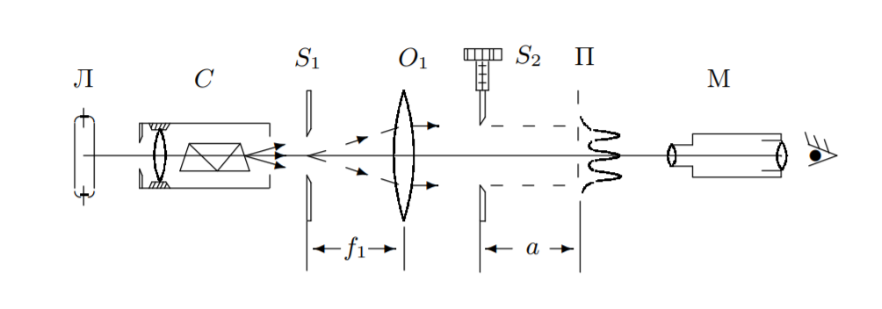
\includegraphics[width=0.7\textwidth]{pics/1.png}
\centering
\caption{Схема установки.}
\end{figure}
Распределение интенсивности света в плоскости П рассчитаем с помощью зон Френеля. При освещении $S_2$ параллельным пучком лучей (плоская зона) зоны Френеля представляют собой плоскости, параллельные краям щели. Результирующая амплитуда в точке наблюдения определеяется суперпозицией колебаний от тех зон Френеля, которые не перекрыты створками щели. Графическое определение результирующей амплитуды производится с помощью векторной диаграммы -- спирали Корню. Суммарная ширина $m$ зон Френеля $z_m$ определяется соотношение
\begin{equation}
z_m = \sqrt{am\lambda},
\end{equation}
где $a$ -- расстояние от щели до плоскости П. Вид наблюдаемой картины определяется \textit{числом Френеля} $\Phi$:
$$
\Phi^2 = \dfrac{D}{\sqrt{a\lambda}}
$$
-- число зон Френеля, которые укладываются в ширине щели $D$. $p = \frac{1}{\Phi^2}$ называется \textit{волновым параметром}. 

\newpage

\subsection{Дифракция Фраунгофера на одной щели}

\begin{wrapfigure}{r}{0.5\textwidth}
  \begin{center}
    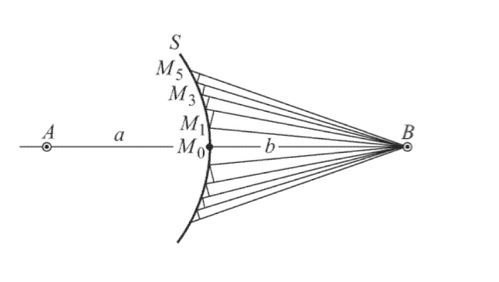
\includegraphics[width = 0.4\textwidth]{pics/2.png}
  \end{center}
  \caption{Построение зон Френеля}
\end{wrapfigure}
Для выкладок ниже нам потребуется знать \textit{принцип Гюйгенса-Френеля}. Он формулируется следующим образом 

\textit{Каждый элемент волнового фронта можно рассматривать как центр  вторичного возмущения, порождающего вторичные сферические волны, а результирующее световое поле  в каждой точке пространства будет определяться интерференцией этих волн.}

Теперь рассмотрим первое применение этого принципа, получившее название \textit{метод зон Френеля}

Для этого рассмотрим действие световой волны действующей из точки $A$ в какой-то точке $B$.

В этом случае можно, взяв точку $M_0$ в качестве центра (см. рис. 1), построить ряд концентрических сфер, радиусы которых начинаются с $b$ и увеличиваются каждый раз на половину длины волны $\lambda/2$. При пересечении с плоским фронтом волны $F$ эти сферы дадут концентрические окружности. Таким образом, на фронте волны появятся кольцевые зоны (зоны Френеля) с радиусами $r_1, r_2$ и т. д.

Из геометрических соображений посчитав, можно получить, что 
\begin{equation}
r_i = i \sqrt{a \lambda}
\end{equation}	
Введем так же обозначение: \textit{число Френеля}
\begin{equation}
\Phi^2 = \dfrac{D}{\sqrt{a\lambda}}
\end{equation}
\begin{wrapfigure}{r}{0.5\textwidth}
  \begin{center}
    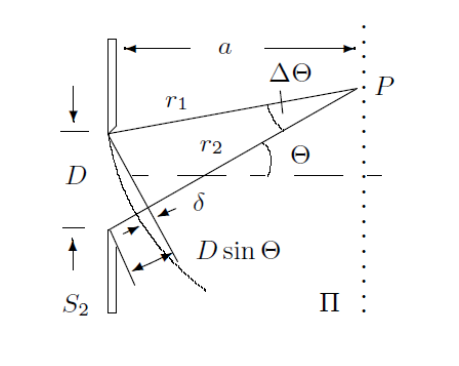
\includegraphics[width = 0.3\textwidth]{pics/3.png}
  \end{center}
  \caption{К фазовым соотношениям при дифракции Фраунгофера}
\end{wrapfigure}
В этом пункте рассмотрим дифракцию, когда ширина щели становится значительно меньше ширины первой зоны Френеля, т.е. если 
\begin{equation}
D \ll\sqrt{a \lambda} 
\end{equation}	
Это условие всегда выполняется при достаточно большом $a$. В этом случае говорят, что \textit{дифракция Фраунгофера}. При выполнении пункта $(2)$ у нас заметно упрощаются фазовые соотношения, что поясняет рис. 2, в итоге с хорошим приближением можно считать, что разность хода между соседними лучами равна 
\begin{equation}
\Delta = r_2 - r_1 \approx D \sin \theta \approx D \cdot \theta
\end{equation}
Здесь предполагается, что $\theta$ достаточно мал.


\subsection{Схема установки}
Дифракцию Фраунгофера можно наблюдать на подобной установке 

\begin{figure}[h]
\begin{center}
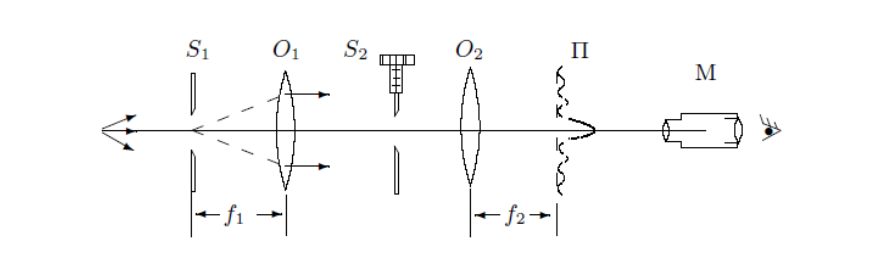
\includegraphics[width = 0.7\textwidth]{pics/4.png}
\caption{Схема установки для пункта 2}
\end{center}
\end{figure}

Объектив здесь нужен для удобства, так как неудобно работать с очень узкими щелями. Дифракционная картина здесь наблюдается в фокальной плоскости объектива $O_2$. 

Посчитав легко определить угловую координату любой темной полосы:
\begin{equation}
\theta_m = \frac{m \lambda}{D}
\end{equation}
И расстояние от центра соответственно 
\begin{equation}
X_m = f_2m\frac{\lambda}{D}
\end{equation}

\subsection{Дифракция Фраунгофера на двух щелях}

Заменим $S_2$ на две щели 

\begin{figure}[h]
\begin{center}
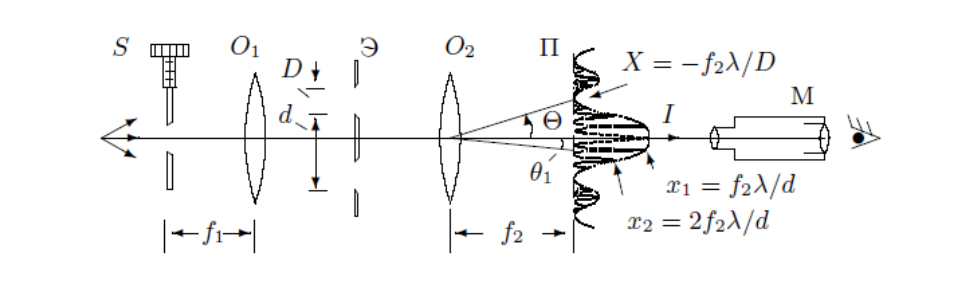
\includegraphics[width = 0.8\textwidth]{pics/5.png}
\caption{Установка для третьего пункта}
\end{center}
\end{figure}

В этом случае легко видеть, что угловая координата максимума будет 
\begin{equation}
\theta_m = \frac{m \lambda}{d}
\end{equation}
И между соседними полосами 
\begin{equation}
\delta x = f_2 \frac{\lambda}{d}
\end{equation}
Так же нетрудно оценить число интерференционных полос укладывающихся в области центрального максимума 
\begin{equation}
n = \frac{2d}{D}
\end{equation}


\subsection{Влияние дифракции на разрешающую способность оптического инструмента}

\begin{figure}[h]
\begin{center}
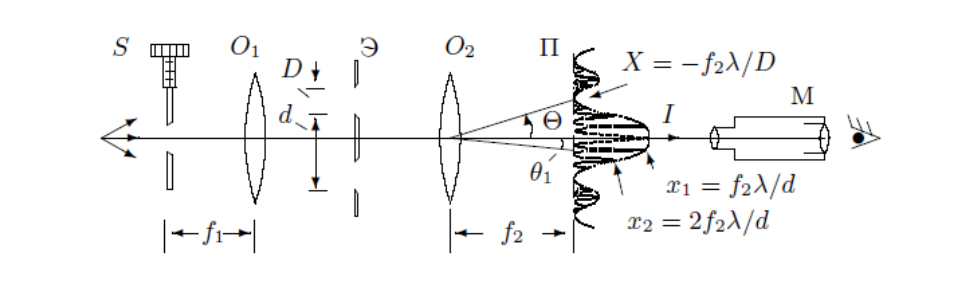
\includegraphics[width = 0.8\textwidth]{pics/5.png}
\caption{Схема установки для пункта 4.}
\end{center}
\end{figure}

Если перед $O_2$ расположить $S_2$, то изображение объекта будет искажено из-за дифракции. Качественной характеристикой этого искажения может служить $\varphi_{min}$ --- минимальное угловое между объектами (источниками). 

\begin{equation}
\varphi = \frac{d}{f_1}
\end{equation}
Из геометрии $l$ между объектами равно 
\begin{equation}
l = \phi \cdot d_2
\end{equation}
\begin{equation}
\dfrac{\lambda}{D_0} = \dfrac{l}{f_2} = \dfrac{d}{f_1}
\end{equation}

\newpage
\section{Результаты измерений и обработка данных}

Соберем схему и подготовим приборы к работе, следуя техническому описанию, расположенному на установке.


\subsection{Часть А}

\subsubsection{Измерения и обработка результатов}

Запишем ширину щели: $ b = 0,360 \pm 0,005 $ мм.

Приближая микроскоп к щели, снимем зависимость координаты микроскопа от числа $ n $ темных полос по формуле $ a_n = x_n - x_0 $, где $ x_0 = 52,9 $ мм --- положение нуля. Результаты занесем в табл. 1 и построим график зависимости величины $ 2\xi_n $ от $ n $. Длина волны зеленого света $ \lambda = 5461 \cdot 10^{-10} $ м. (Формула 1)

\begin{table}[h!]
\caption{Зависимость координаты микроскопа от числа $ n $ темных полос}
\begin{center}
	\begin{tabular}{|c|c|c|c|}
		\hline
		$ x_n $, мм & $ n $ & $ a_n $, мм & $ \xi_n $, мм\\
		\hline
		539 & 5 & 6 & 0.404 \\
		537 & 4 & 8 & 0.418 \\
		535 & 3 & 10 & 0.404 \\
		531 & 2 & 12 & 0.362 \\
		\hline
	\end{tabular}

\end{center}
\label{}
\end{table}

	\begin{center}
		\begin{tikzpicture}[scale = 1.0]
		\begin{axis}[
		axis lines = left,
		ylabel = {$\xi$},
		xlabel = {n},
		minor grid style={black, line width=0.05pt},
		major grid style={solid,black, line width=0.3pt},
		xmin=1, xmax=6,
		ymin=0, ymax=0.5,
		ymajorgrids = true,
		xmajorgrids = true,
		yminorgrids = true,
		xminorgrids = true,
		minor tick num = 3
		]
		\addplot+[only marks ] plot[error bars/.cd, y dir=both, y explicit]
		coordinates {
			(2,0.362) +- (0.02,0.02)
			(3,0.404) +- (0.02,0.02)
			(4,0.418) +- (0.02,0.02)
			(5,0.404) +- (0.02,0.02)
		};

		\addplot[blue, ultra thick, domain=0:8]{0.36};
		\end{axis}

		\end{tikzpicture}

		График зависимости суммарной ширины зон Френеля от их числа
\end{center}

Таким образом, ширина примерно совпадает с шириной щели и является постоянной величиной. "<Сдвиг"> объясним неточностью в измерении нуля.

\subsection{Часть Б}
Величина щели по винту равна $ b =  0,5 \pm 0,03 $ мм. Фокусное расстояние линзы $ f_2 = 10.0 $ см.

Измерим с помощью винта поперечного перемещения микроскопа координаты $ X_m $ нескольких дифракционных минимумов. Здесь $ x_m $ --- измерения, которые затем умножаем на $ \alpha = 0,02 $ мм --- цену деления винта, т.е. $ X_m = \alpha x_m $.
 Результаты занесем в табл. 2 и построим график зависимости минимумов от их номеров. \\

\begin{minipage}{0.47\textwidth}


\begin{center}
		\begin{tabular}{|c|c|c|}
			\hline
			$ x_m $ & $ X_m $, мм & $ m $ \\
			\hline
			-9.0 & -0.090 & -4\\
			-5.0 & -0.050 & -3\\
			-2.5 & -0.025 & -2\\
			-1.0 & -0.010 & -1\\
			3.0 & 0.030 & 1\\
			5.0 & 0.050 & 2\\
			7.0 & 0.070 & 3\\
			9.0 & 0.090 & 4\\
			\hline
		\end{tabular}
	\end{center}

\end{minipage}
\begin{minipage}{0.47\textwidth}
\begin{center}
		\begin{tikzpicture}[scale = 1.0]
		\begin{axis}[
		axis lines = left,
		ylabel = {$X_m$},
		xlabel = {f(m)},
		minor grid style={black, line width=0.05pt},
		major grid style={solid,black, line width=0.3pt},
		xmin=-5, xmax=5,
		ymin=-0.1, ymax=0.1,
		ymajorgrids = true,
		xmajorgrids = true,
		yminorgrids = true,
		xminorgrids = true,
		minor tick num = 4
		]
		\addplot+[only marks ] plot[error bars/.cd, y dir=both, y explicit]
		coordinates {
			(-4,-0.09)
			(-3,-0.05)
			(-2,-0.025)
			(-1,-0.01)
			(1,0.03)
			(2,0.05)
			(3,0.07)
			(4, 0.09)
		};

		\addplot[blue, thick, domain=-5:5]{0.023*x + 0.01 };
		\end{axis}

		\end{tikzpicture}

\end{center}
\end{minipage}

\begin{center}
Зависимость минимумов от их номера $ m $
\end{center}

Из графика получаем, что угол наклона $ a = (23,0 \pm 1,2) \cdot 10^{-4} $ мм. Это и есть расстояние $ \Delta X $ между соседними максимумами. Из формулы 4 мы получаем, что

\begin{equation}
b_{\text{э}}= \frac{X_m}{m} = \dfrac{\lambda}{b_{\text{э}}} f_2 b_{\text{э}} = 2 \cdot \dfrac{\lambda}{a} f_2 = 0,502 \pm 0,007 \; мм.
\end{equation}

Таким образом, наши значения для $ b $ и $ b_{\text{э}} $ близки.
\
  \begin{center}
    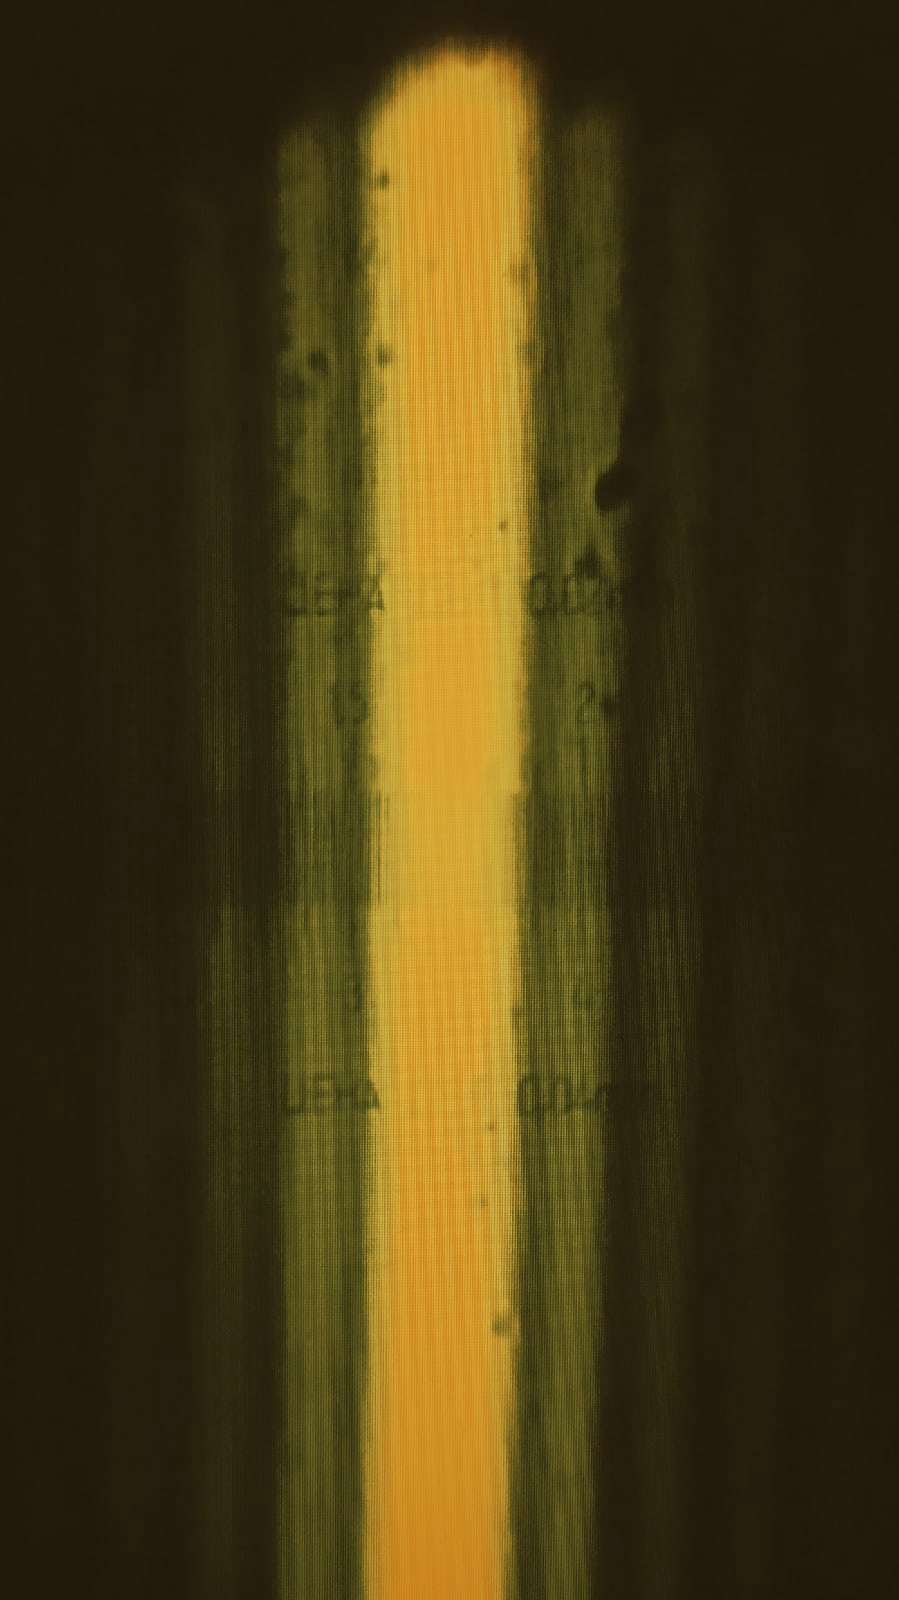
\includegraphics[scale = 0.2]{pics/7.png}\\

    Дифракционная картина на одной щели
  \end{center}


\subsection{Часть В}

Получим на экране дифракционную картину и проведем измерения. Получим для 1 и 2 максимума слева и справа соответственно координаты на винте $ x_m $, а затем получим $ X_m = \alpha x_m $ аналогично предыдущему пункту.

\begin{center}
\begin{tabular}{|c|c|c|c|c|}
	\hline
	$m$ & -2 & -1 & 1 & 2 \\
	\hline
	$x_m$ & -1,55 & -1,6 & 0.7 & 0.8 \\
	\hline
	$Х_m$, мм & -0.031 & -0.032 & 0.015 & 0.018 \\
	\hline
\end{tabular}

\begin{center}
Измерения максимумов на двух щелях\
\end{center}

\end{center}


 Ширина главных максимумов $  \delta x  = 3 (x_{1} - x_{-1} )= 0,042 $ мм, где 3 --- число наблюдаемых светлых полос. Из формулы $5$ получаем расстояние между щелями

 \begin{equation}\label{}
 d = f_2 \dfrac{\lambda}{\delta x} = 0,144 \pm 0,006 \; мм
 \end{equation}

Это примерно сходится с измеренной непосредственно $ b_0 \approx 0,07 $. Так как эта же ширина равна $ \frac{2f_2 \lambda}{b}$

 \begin{equation}\label{}
 b = \dfrac{2 f_2 \lambda}{d} = 0,082 \pm \;0,004 мм
 \end{equation}

 Из формулы 10 мы получаем $ n = \dfrac{2\cdot 0,134}{0,089} \approx 3,01 \pm 0,08 $, что сходится с наблюдениями.

  \begin{center}
    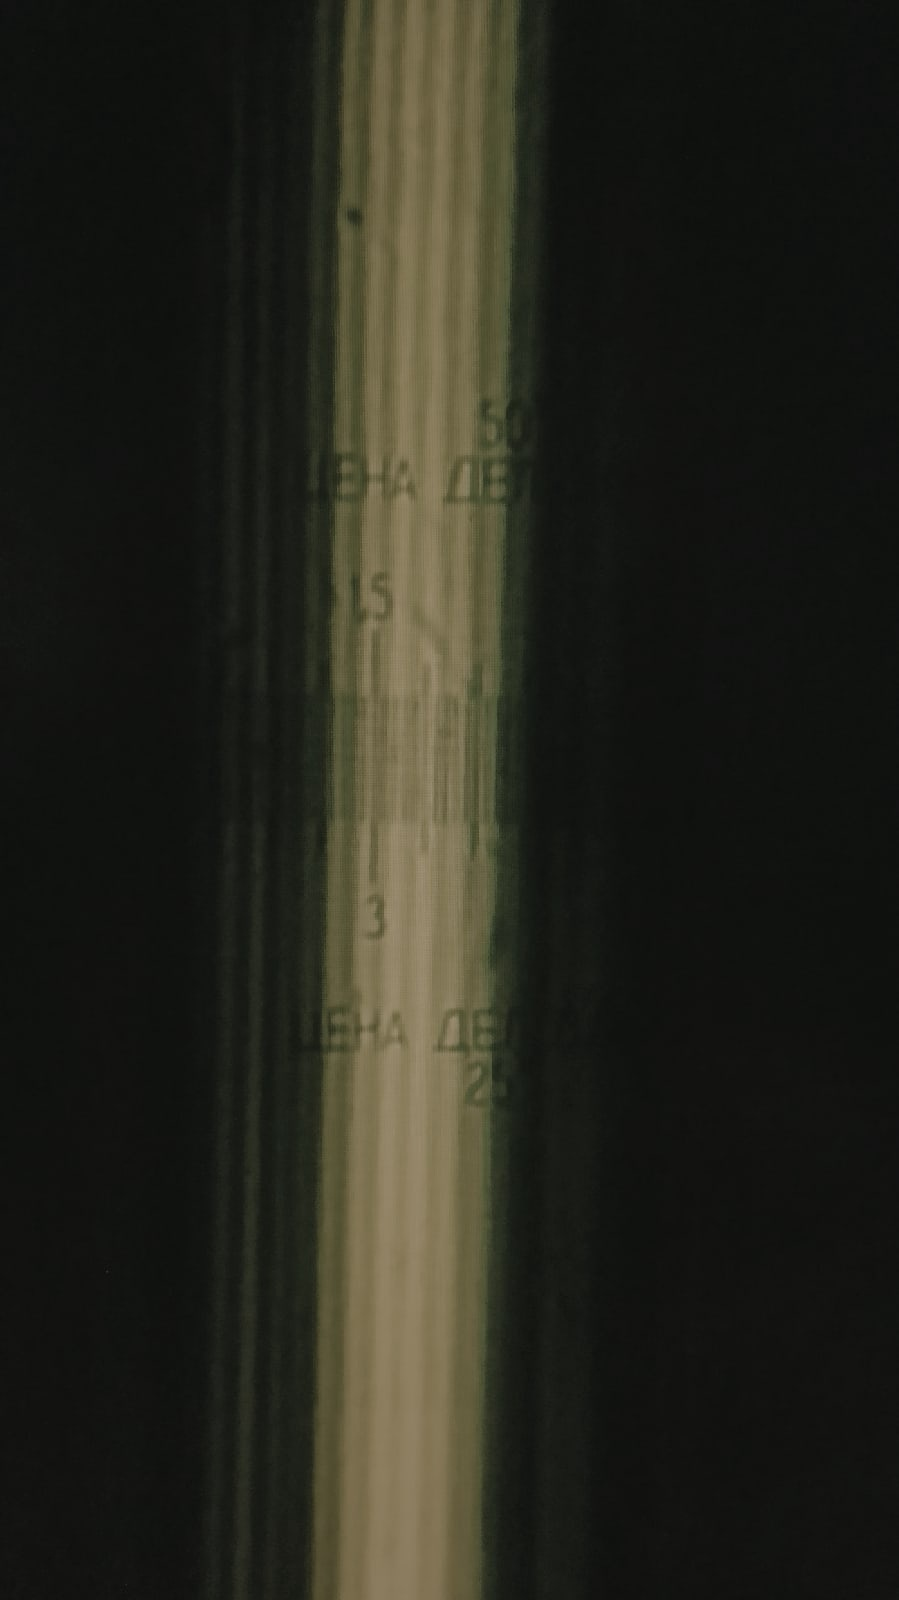
\includegraphics[scale=0.25]{pics/8.png}\\

    Дифракционная картина на двух щелях
  \end{center}

\subsection{Часть Г}
\begin{enumerate}
\item Собрали схему, изменив в схеме из предыдущего пункта только $S$.
\item Поставили между линзами щель $S_2$ и уменьшая ее ширину наблюдать ухудшение изображения. Подобрать ширину $S_2$ так, чтобы изображения почти сливались.
\[D_0 = (0,060 \pm 0,005)\text{мм}\]


Погрешность берем как половину цены деления.
В итоге получаем, что выполнено соотношение $(13)$.
\item Поставить двойную щель и измерить расстояние между щелями и толщину самих щелей.
\[d = (1,00 \pm 0,01) \text{мм}\]
\[D = (0,20 \pm 0,01) \text{мм}\]

Погрешность берем как половину цены деления.
\end{enumerate}

\section{Выводы}

По ходу выполнения данной работы были изучены два типа дифракции: Френеля и Фраунгофера.
Изучение происходило при различных размерах щелей. Экспериментально проверили теоретические формулы:

\begin{equation}
b_{\text{э}}= \frac{X_m}{m} = \dfrac{\lambda}{b_{\text{э}}} f_2 b_{\text{э}} = 2 \cdot \dfrac{\lambda}{a} f_2 = 0,502 \pm 0,007 \; мм.
\end{equation}

\begin{equation}
n = \frac{2d}{D} = 3,01 \pm 0,08\ ,
\end{equation}

что сходится с наблюдениями.

\section{Литература}

\begin{enumerate}

\item Лабораторный практикум по общей физике. В 3 т. Том 2. Оптика: учебное пособие

\item http://mathhelpplanet.com (МНК и регрессионный анализ)


\end{enumerate}	

\end{document}
